% ── Paleta Terracota PDF ──
\definecolor{docereblack}{HTML}{3a2418}
\definecolor{docerewhite}{HTML}{FFFFFF}

\definecolor{docere-link}{HTML}{8a4030}
\definecolor{docere-cite}{HTML}{503020}
\definecolor{docere-url}{HTML}{8a4030}
\usepackage{amsmath}
\usepackage{amssymb}
\usepackage[version=4]{mhchem}
\usepackage{graphicx}
\usepackage{pdfpages}

% ── Font: Atkinson Hyperlegible ──
\usepackage[T1]{fontenc}
\usepackage[sfdefault]{atkinson}

\usepackage{microtype}
\usepackage{enumitem}
\usepackage{caption}
\usepackage{longtable}
\usepackage{booktabs}

% ── Paragraph styling ──
\usepackage{parskip}
\setlength{\parskip}{0.8em}
\raggedright
\usepackage{setspace}
\setstretch{1.5}

\usepackage{tikz}
\usepackage{tcolorbox}
\tcbuselibrary{skins, breakable, raster}

\definecolor{icfesletra}{HTML}{a06050}
\definecolor{icfesbg}{HTML}{fdf5f2}
\definecolor{icfesborder}{HTML}{a06050}
\definecolor{icfescircle}{HTML}{a06050}

% ── Table styling ──
\definecolor{icfesheader}{HTML}{ede0d8}
\definecolor{icfestext}{HTML}{503020}
\definecolor{icfeveryodd}{HTML}{fdf5f2}
\definecolor{icfeveryeven}{HTML}{f6eeea}
\definecolor{icfestabletext}{HTML}{3a2418}
\definecolor{icfestablecapbg}{HTML}{f0ddd4}
\newcommand{\circletter}[1]{%
  \tikz[baseline=(char.base)]{%
    \node[fill=icfescircle, text=white, circle, minimum size=1.8em, inner sep=0pt, font=\bfseries\small] (char) {#1};%
  }%
}

\newcommand{\colorframe}[3]{%
  \tikz[baseline=(X.base)]{%
    \node[fill=#1, draw=#2, rounded corners=2pt, inner xsep=4pt, inner ysep=1pt, font=\small] (X) {#3};%
  }%
}

\definecolor{currentsectionbg}{HTML}{fdf5f2}
\definecolor{currentsectionborder}{HTML}{a06050}

\newcommand{\setcolorsection}[2]{%
  \definecolor{currentsectionbg}{HTML}{#1}%
  \definecolor{currentsectionborder}{HTML}{#2}%
}

% ── Docere Interactive Cards (PDF) ──
\newtcolorbox{docerecard}{
  colback=white,
  colframe=black!10,
  arc=4pt,
  boxrule=0.5pt,
  left=12pt,
  right=12pt,
  top=8pt,
  bottom=8pt,
  before skip=12pt,
  after skip=12pt,
  breakable,
  enhanced,
  drop fuzzy shadow=black!5
}

% ── Docere Question Cards (PDF) ──
\definecolor{basica-color}{HTML}{2ecc71}
\definecolor{basica-bg}{HTML}{eafaf1}
\definecolor{media-color}{HTML}{f39c12}
\definecolor{media-bg}{HTML}{fef5e7}
\definecolor{dificil-color}{HTML}{e74c3c}
\definecolor{dificil-bg}{HTML}{fdedec}

\newtcolorbox{preguntabasica}[1][]{
  colback=basica-bg,
  colframe=basica-color,
  fonttitle=\bfseries,
  coltitle=white,
  arc=4pt,
  boxrule=1pt,
  #1
}

\newtcolorbox{preguntamedia}[1][]{
  colback=media-bg,
  colframe=media-color,
  fonttitle=\bfseries,
  coltitle=white,
  arc=4pt,
  boxrule=1pt,
  #1
}

\newtcolorbox{preguntadificil}[1][]{
  colback=dificil-bg,
  colframe=dificil-color,
  fonttitle=\bfseries,
  coltitle=white,
  arc=4pt,
  boxrule=1pt,
  #1
}

\addtokomafont{section}{\normalfont\Large\bfseries\color{docereblack}}

\renewcommand{\sectionlinesformat}[4]{%
  \begin{tcolorbox}[
    colback=currentsectionbg,
    colframe=currentsectionborder,
    arc=3pt,
    boxrule=0.5pt,
    left=8pt,
    right=8pt,
    top=4pt,
    bottom=4pt,
    before skip=0pt,
    after skip=0pt,
    nobeforeafter,
    ]
    #4%
  \end{tcolorbox}%
}

\AtBeginDocument{
  % ── Apply optimized contrast ──
  \pagecolor{docerewhite}
  \color{docereblack}
  
  \setlength{\abovedisplayskip}{1em}
  \setlength{\belowdisplayskip}{1em}
  \setlength{\abovedisplayshortskip}{0.5em}
  \setlength{\belowdisplayshortskip}{0.5em}
  \frontmatter
  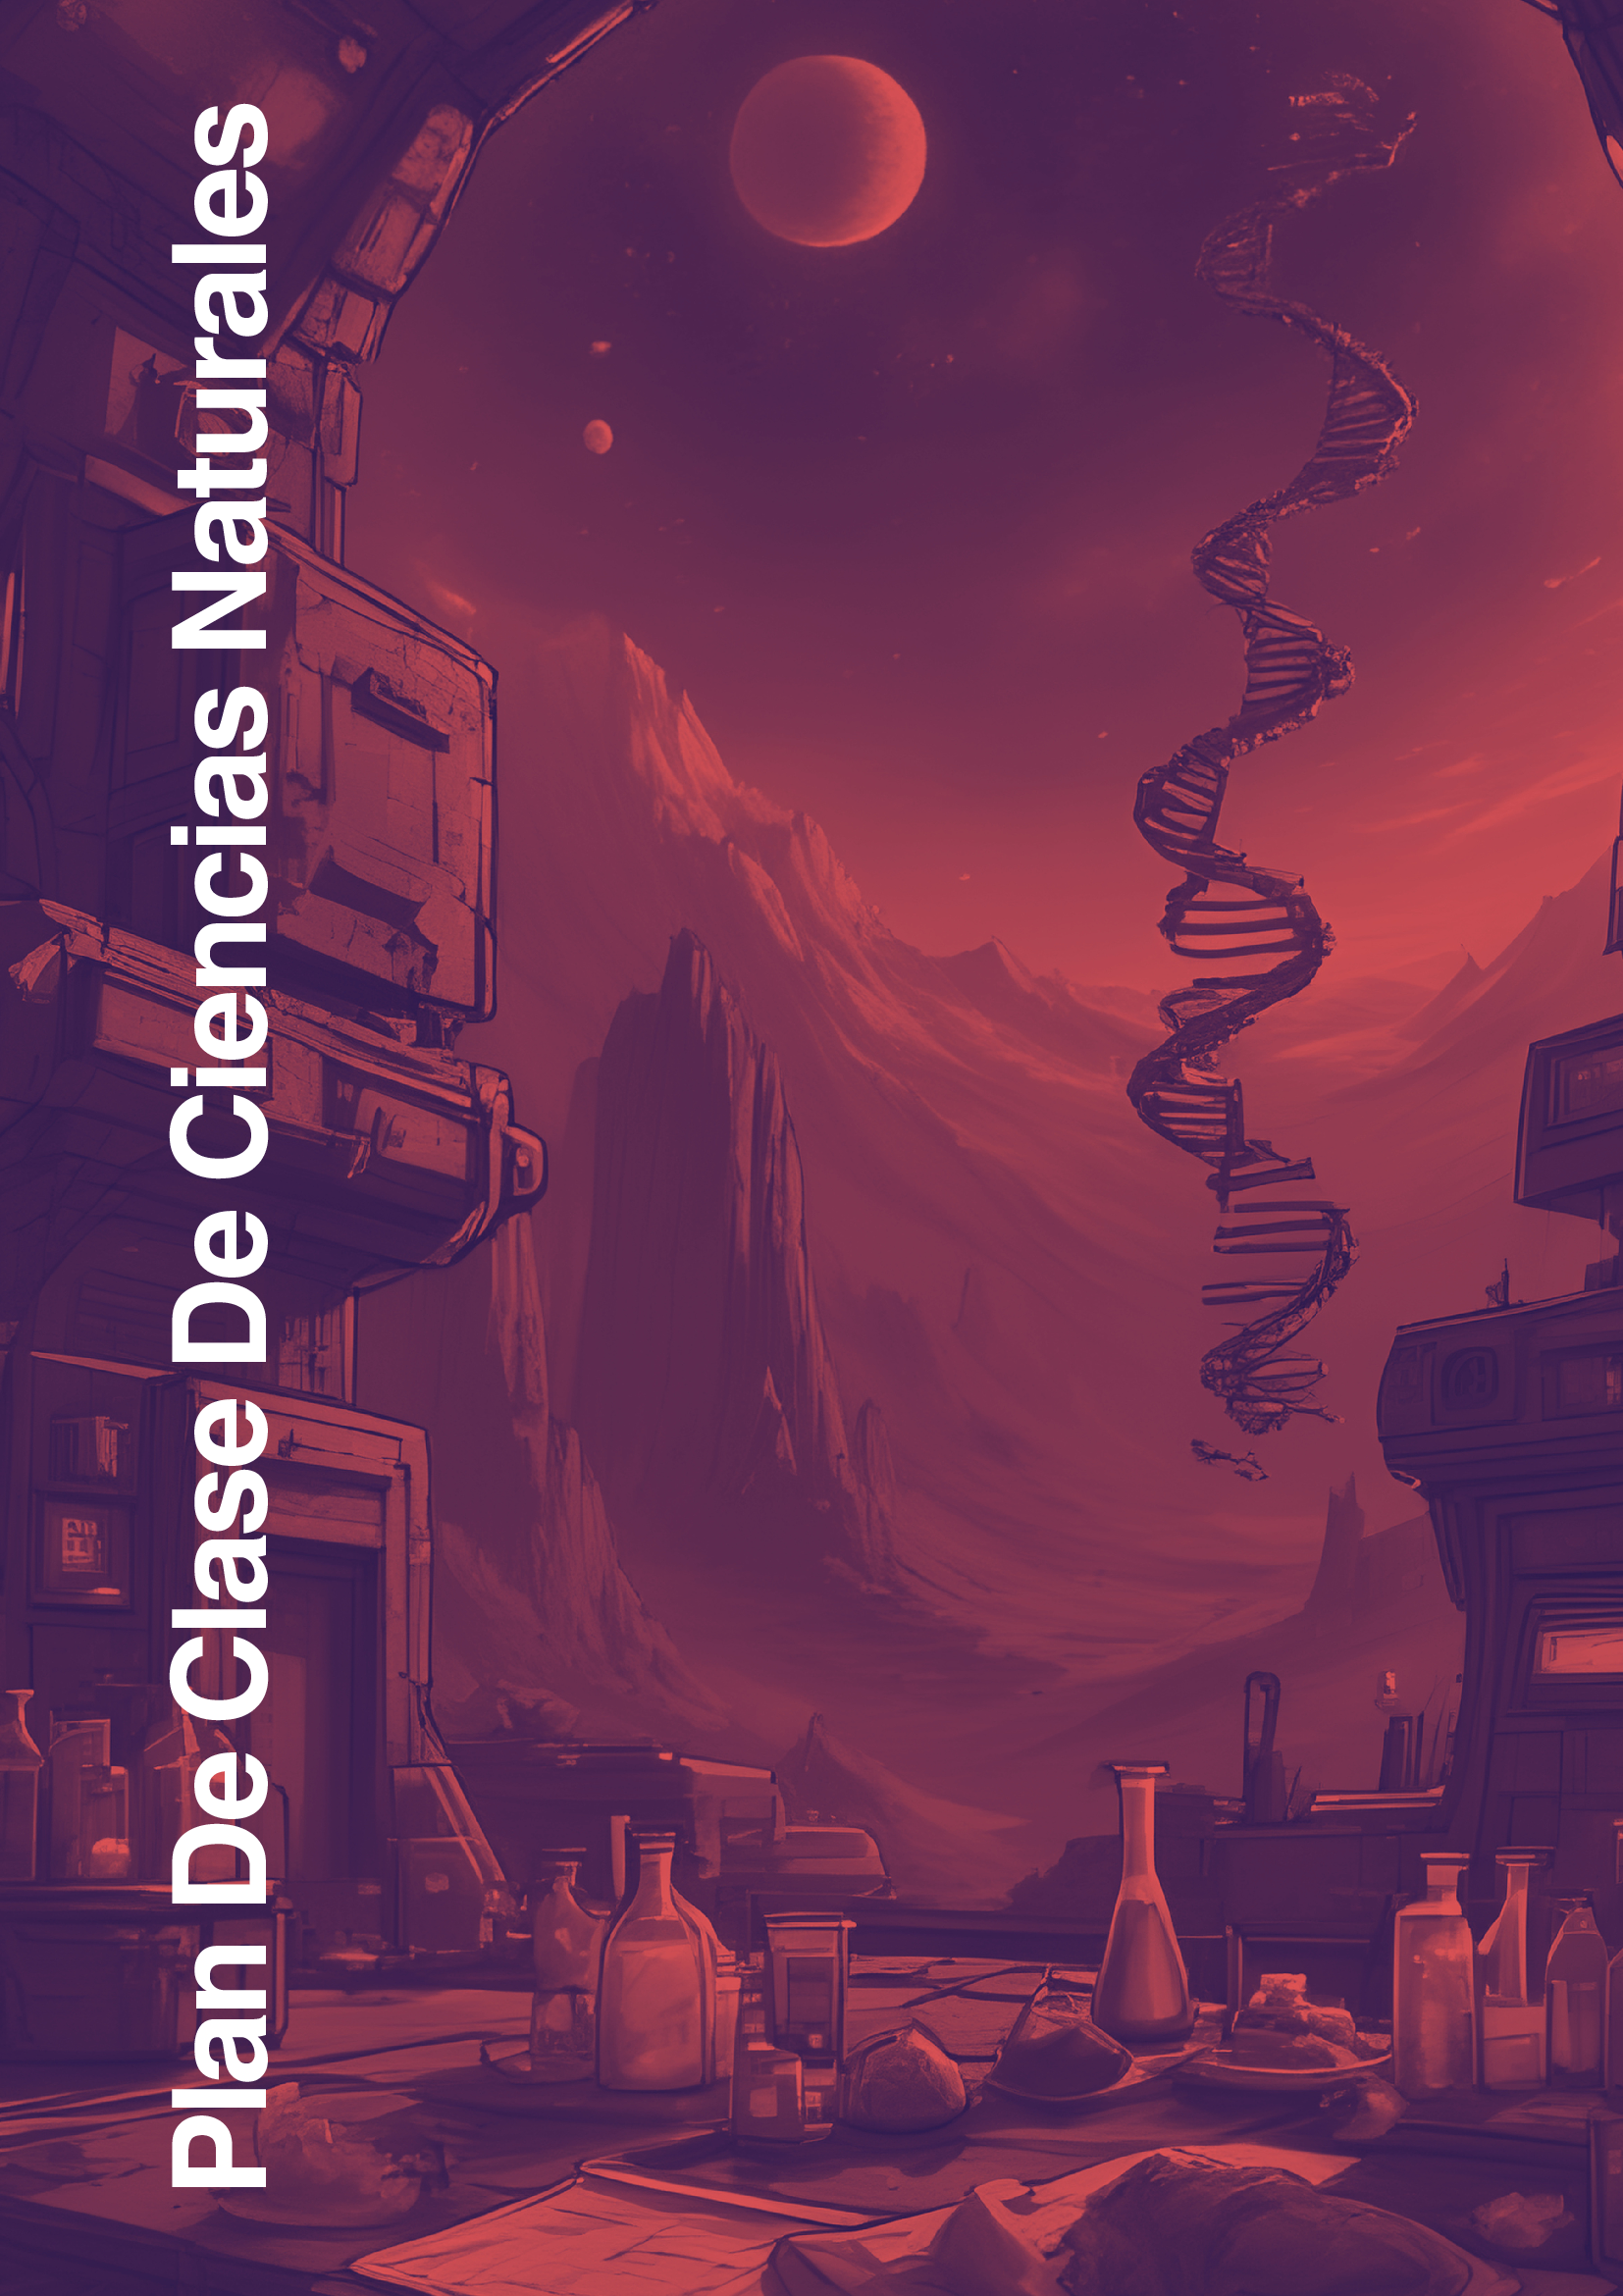
\includepdf[pages=-, fitpaper]{Portada.pdf}
  \mainmatter
  \pagestyle{plain}
}
